\documentclass[12pt,letterpaper]{article}
\usepackage[top=2cm, bottom=4.5cm, left=2.5cm, right=2.5cm]{geometry}
\usepackage{amsmath,amsthm,amsfonts,amssymb,amscd}
\usepackage{enumerate}
\usepackage{fancyhdr}
\usepackage{xcolor}
\usepackage{graphicx}
\usepackage{hyperref}
\usepackage{pgfplots}
\pgfplotsset{width=15cm}

\hypersetup{%
  colorlinks=true,
  linkcolor=blue,
  linkbordercolor={0 0 1}
}

\setlength{\parindent}{0.0in}
\setlength{\parskip}{0.05in}

% Edit these as appropriate
\newcommand\course{ELEC 2600}
\newcommand\hwnumber{3}                  % <-- homework number
\newcommand\NetIDa{Huang Daoji}           % <-- NetID of person #1
\newcommand\NetIDb{20623420}

\pagestyle{fancyplain}
\headheight 35pt
\lhead{\NetIDa \\ \NetIDb}
\chead{\textbf{\Large Homework \hwnumber}}
\rhead{\course \\ \today}
\lfoot{}
\cfoot{}
\rfoot{\small\thepage}
\headsep 1.5em

\begin{document}

\section*{Problem 1}
    \subsection*{a}
        From the joint pmf, we have
        \begin{equation*}
            \begin{aligned}
                c + 0.1 + 0.1 + 0.2 + 0.1 + 0.2 + 0.1 + 0.1 &= 1 \\
                c &= 0.1 \\
            \end{aligned}
        \end{equation*}
    \subsection*{b}
        From definition of joint cdf, $F_{XY}(2, 1)$ will be
        \begin{equation*}
            \begin{aligned}
                F_{XY}(2, 1) &=  \sum_{x \leq 2,\ y \leq 1} p_{XY}(j, k) \\
                &= 0.1 + 0.1 + 0.2 + 0.1 \\
                &= 0.5 \\
            \end{aligned}
        \end{equation*}
    \subsection*{c}
        From the table of pmf, by summing up the $p_{XY}(j, k)$ in each row / column, we have
        \begin{center}
            \begin{tabular}{| c | c | c | c | c | c |}
                \hline
                $j$  & 1 & 2 & 3 & 4 & otherwise\\
                \hline
                $P_{X}(j)$ & 0.3 & 0.3 & 0.2 & 0.2 & 0 \\
                \hline
            \end{tabular}
        \end{center}
        \begin{center}
            \begin{tabular}{| c | c | c | c | c |}
                \hline
                $k$  & 0 & 1 & 2 & otherwise\\
                \hline
                $P_{Y}(k)$ & 0.3 & 0.5 & 0.2 & 0 \\
                \hline
            \end{tabular}
        \end{center}
    \subsection*{d}
        No, a counterexample would be $(4, 1)$, where $P_{XY}(4, 1) \not= P_{X}(4) \times P_{Y}(1)$
    \subsection*{e}
        Yes, by calculating the covarience of $X, Y$, we have
        \begin{equation*}
            \begin{aligned}
                Cov(X, Y) &= E(XY) - E(X)E(Y) \\
                &= 2.2 - 2.07 \\
                &= 0.13 \not= 0, \\
            \end{aligned}
        \end{equation*}
        which means $X, Y$ are correlated.
    \subsection*{f}
        First, calculate standard variation of $X, Y$
        \begin{equation*}
            \begin{aligned}
                \sigma_{X} &= (E(X^{2}) - (E(X))^{2})^{1/2} \\
                &= (6.5 - 2.3^{2})^{1/2} \\
                &= 1.1 \\
            \end{aligned}
        \end{equation*}
        \begin{equation*}
            \begin{aligned}
                \sigma_{Y} &= (E(X^{2}) - (E(X))^{2})^{1/2} \\
                &= (1.3 - 0.9^{2})^{1/2} \\
                &= 0.7 \\
                \\
                r &= Cov(X, Y) / \sigma_{X}\sigma_{Y} \\
                &= 0.1688 \\
            \end{aligned}
        \end{equation*}
    \subsection*{g}
        From the marginal pmf of Y, we have $P(Y < 1) = 0.3$, then the conditional pmf of $X$ can be calculated using $P_{X | Y < 1}(j) = P(j, Y < 1) / P(Y < 1)$, We have
        \begin{center}
            \begin{tabular}{| c | c | c | c | c | c |}
                \hline
                $j$  & 1 & 2 & 3 & 4 & otherwise\\
                \hline
                $P_{X | Y < 1}(j)$ & 1/3 & 1/3 & 0 & 1/3 & 0 \\
                \hline
            \end{tabular}
        \end{center}
    \subsection*{h}
        From the conditional pmf in $g$, the conditional expected value of $X$ is
        \begin{equation*}
            \begin{aligned}
                E(X | Y < 1) &= \sum_{j} j * P_{X | Y < 1}(j) \\
                &= 7/3 \\
            \end{aligned}
        \end{equation*}

\section*{Problem 2}
    \subsection*{a}
        From the joint pmf of $X, Z$, we have
        \begin{equation*}
            \begin{aligned}
                P_{X}(x) &= \sum_{z = x}^{+\infty} \frac{3^{z}}{x!(z - x)!} 0.4^{x} 0.6^{z - x} e^{-3} \\
                &= \frac{1.2^{x}}{x!} e^{-3} \sum_{t = 0}^{+\infty}  \frac{1.8^{t}}{t!}\quad (let\ t = z - x) \\
                &= \frac{1.2^{x}}{x!}e^{-1.2} \\
            \end{aligned}
        \end{equation*}
        It belongs to Poisson distribution with mean 1.2
    \subsection*{b}
        From the joint pmf of $X, Z$, we have
        \begin{equation*}
            \begin{aligned}
                P_{Z}(z) &= \sum_{x = 0}^{z} \frac{3^{z}}{x!(z - x)!} 0.4^{x} 0.6^{z - x} e^{-3} \\
                &= \frac{3^{z}}{z!}e^{-3} \sum_{x = 0}^{z} \frac{z!}{x!(z - x)!} 0.4^{x} 0.6^{z - x} \\
                &= \frac{3^{z}}{z!}e^{-3} \\
            \end{aligned}
        \end{equation*}
        It belongs to Poisson distribution with mean 3
    \subsection*{c}
        For $Z = X + Y$, we have
        \begin{equation*}
            \begin{aligned}
                P_{Y}(y) &= \sum_{x = 0}^{+\infty} \frac{3^{x + y}}{x!y!} 0.4^{x} 0.6^{y} e^{-3} \\
                &= \frac{1.8^{y}}{y!} e^{-3} \sum_{x = 0}^{+\infty} \frac{3^{x}}{x!} 0.4^{x} \\
                &= \frac{1.8^{y}}{y!} e^{-1.8} \\
            \end{aligned}
        \end{equation*}
        It belongs to Poisson distribution with mean 1.8
    \subsection*{d}
        No, a counterexample will be $(x, z) = (1, 0)$, for neither of $P_{X}(1), P_{Z}(0)$ equals zero, but by definition $P_{X, Z}(1, 0) = 0$
    \subsection*{e}
        Yes, for
        \begin{equation*}
            \begin{aligned}
                P_{X, Y}(x, y) &= P_{X, Z}(x, x + y)\quad (by\ definition) \\
                &= \frac{3^{x + y}}{x!((x + y) - x)!} 0.4^{x} 0.6^{(x + y) - x} e^{-3} \\
                &= \frac{3^{x + y}}{x!y!} 0.4^{x} 0.6^{y} e^{-3} \\
                &= \frac{1.2^{x}}{x!}e^{-1.2} \times \frac{1.8^{y}}{y!} e^{-1.8} \\
                &= P_{X}(x) \times P_{Y}(y) \\
            \end{aligned}
        \end{equation*}
    \subsection*{f}
        From the pmf of $X, Z$ and marginal pmf of $Z$, we have
        \begin{equation*}
            \begin{aligned}
                P_{X | Z}(x) &= (\frac{3^{z}}{x!(z - x)!} 0.4^{x} 0.6^{z - x} e^{-3}) / (\frac{3^{z}}{z!}e^{-3}) \\
                &= \frac{z!}{x!(z - x)!} 0.4^{x} 0.6^{z - x},
            \end{aligned}
        \end{equation*}
        which belongs to binomial distribution with paremeter $(n, p) = (z, 0.4)$.
    \subsection*{g}
        From the result in $(f)$, the conditional expectation of $X$ is $E[X | Z] = 0.4Z$.

\section*{Problem 3}
    \subsection*{a}
        The red region is where pdf of $X, Y$ is non-zero, which is the intersetion of two functions: $y = x^{2}$ and $y = 1$. \\
        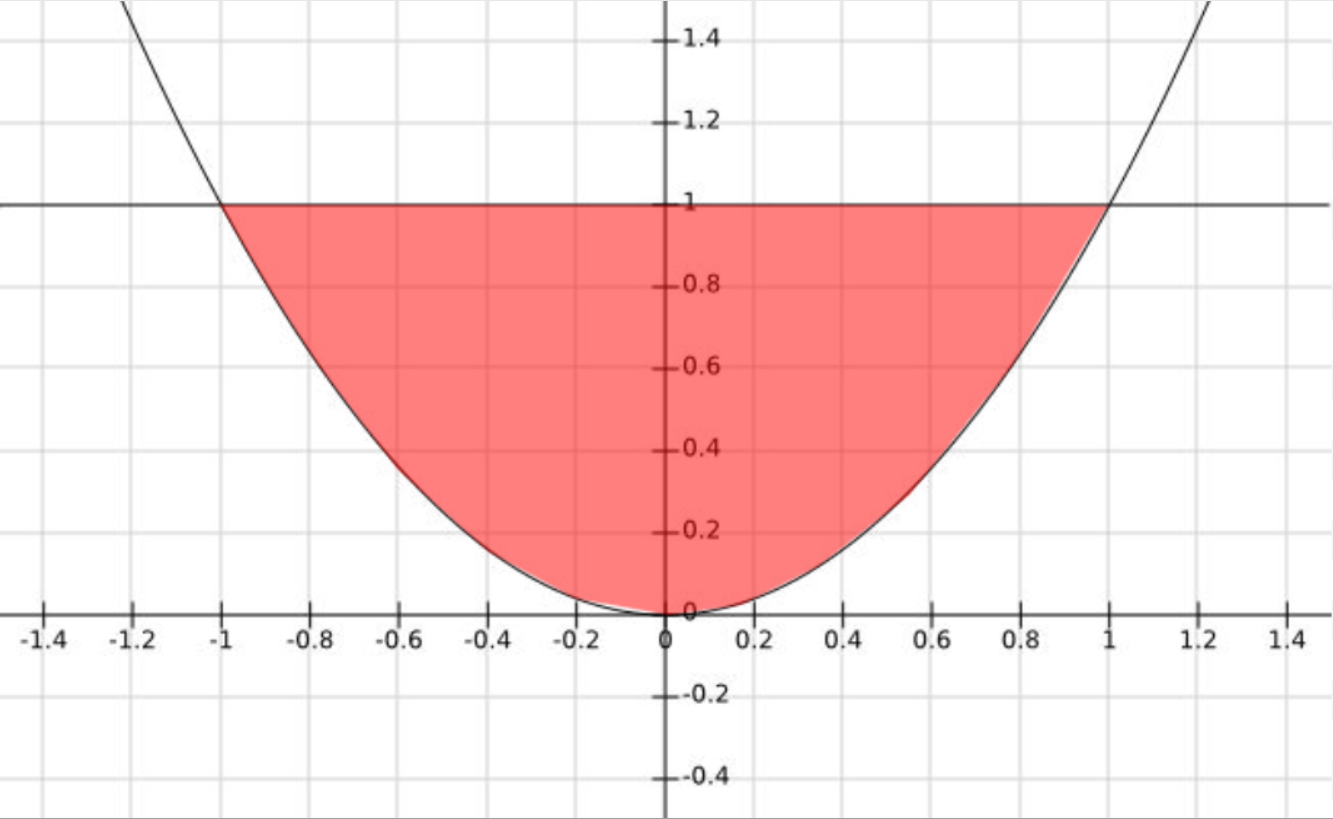
\includegraphics[scale=0.6]{pdf.png}
    \subsection*{b}
        From the property that pdf intergates to one, we have
        \begin{equation*}
            \begin{aligned}
                \iint f_{X, Y}(x, y)\ dxdy &= 1 \\
                \iint_{S} c dxdy &= 1 \\
                c\int_{-1}^{1} \int_{x^{2}}^{1} dy\ dx &= 1 \\
                c \int_{-1}^{1} (1 - x^{2})\ dx &= 1 \\
                c (x - \frac{1}{3}x^{3})|_{-1}^{1} &= 1 \\
                c &= \frac{3}{4} \\
            \end{aligned}
        \end{equation*}
    \subsection*{c}
        For any $x \not\in [-1, 1]$, the pdf of $X$ is zero. For $x \in [-1, 1]$, we have
        \begin{equation*}
            \begin{aligned}
                f_{X}(x) &= \int f_{X, Y}(x, y) dy \\
                &= \int_{x^{2}}^{1} \frac{3}{4} dy \\
                &= \frac{3}{4}(1 - x^{2}) \\
            \end{aligned}
        \end{equation*}
        For any $y \not\in [0, 1]$, the pdf of $Y$ is zero. For $y \in [0, 1]$, we have
        \begin{equation*}
            \begin{aligned}
                f_{Y}(y) &= \int f_{X, Y}(x, y) dx \\
                &= \int_{-y^{1/2}}^{y^{1/2}} \frac{3}{4} \\
                &= \frac{3}{2} y^{1/2} \\
            \end{aligned}
        \end{equation*}
    \subsection*{d}
        By definition,
        \begin{equation*}
            \begin{aligned}
                f_{Y | X}(y | x) &= \frac{f_{X, Y}(x, y)}{f_{X}(x)} \\
                &= \frac{3/4}{3/4 (1 - x^{2})} \\
                &= \frac{1}{1 - x^{2}} \\
            \end{aligned}
        \end{equation*}
        only for $y \in [x^{2}, 1]$, otherwise 0.
        \\
        {\center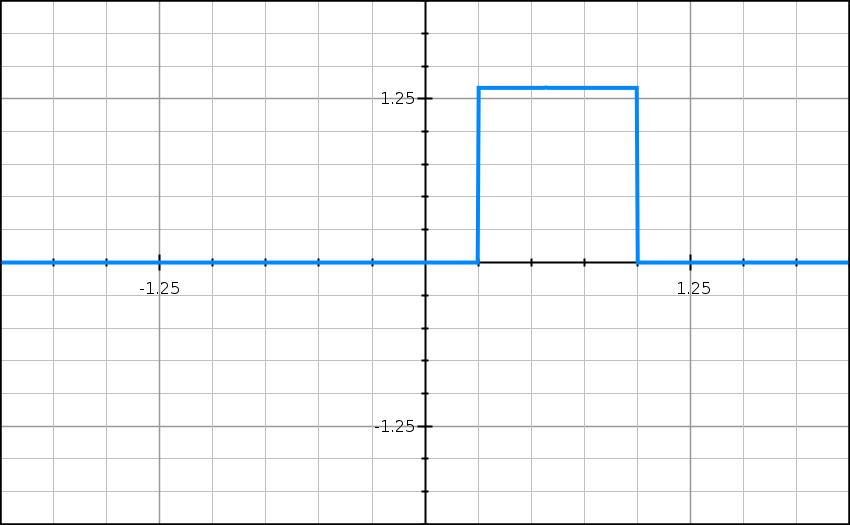
\includegraphics[scale=0.3]{graph.png}}
    \subsection*{e}
        Notice that $Y$ belongs to uniform distribution in $[x^{2}, 1]$ once $X$ is given. We have $E[Y|X] = \frac{1}{2}(1 + x^{2})$ for $y \in [0, 1]$, otherwise 0. \\
        {\center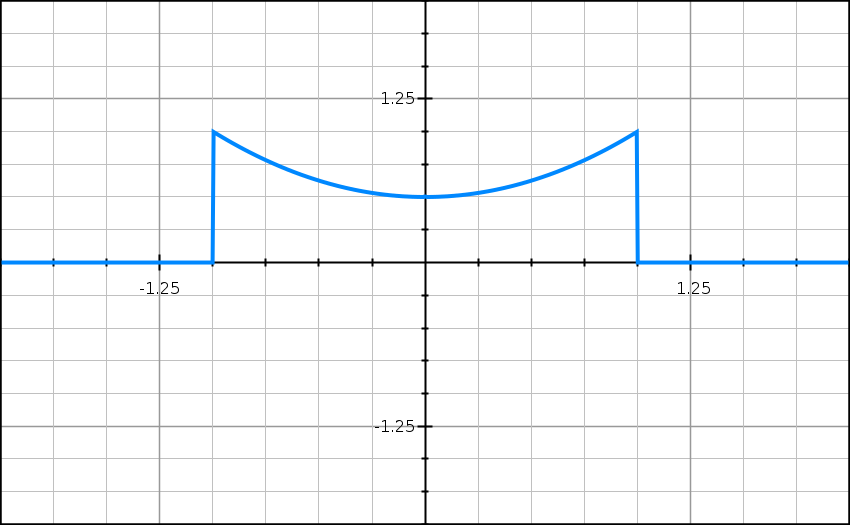
\includegraphics[scale=0.3]{graph2.png}}

\section*{Problem 4}
    \subsection*{a}
        From the fact that $X, Y$ are independent, we have
        \begin{equation*}
            \begin{aligned}
                f_{X, Y}(x, y) &= f_{X}(x) f_{Y}(y) \\
                &= \frac{1}{15 - 5} \times \frac{1}{20 - 5} \\
                &= \frac{1}{150} \\
            \end{aligned}
        \end{equation*}
        for $x \in [5, 15]$ and $y \in [5, 20]$, otherwise 0.
        The region where PDF is non zero is the rectangle $ABCD$.
        {\center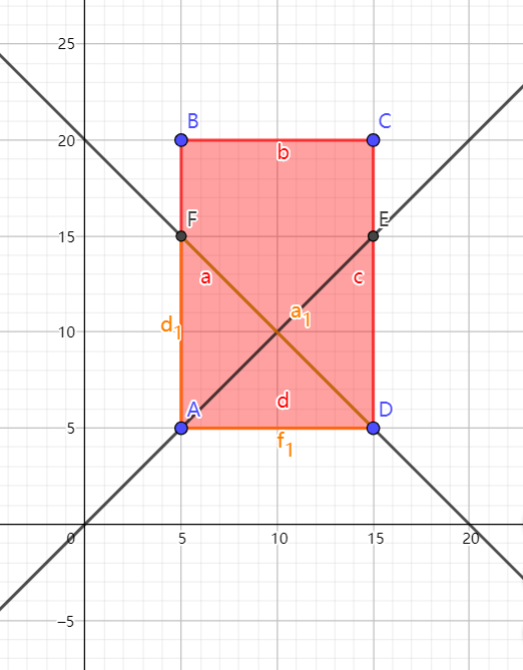
\includegraphics[scale=0.7]{rect.png}}
    \subsection*{b}
        The probability of $Y > X$ is the space ratio of polygon $ABCE$ to rectangle $ABCD$, which is $\frac{2}{3}$
    \subsection*{b}
        The probability of $X + Y < 20$ is the space ratio of triangle $ADF$ to rectangle $ABCD$, which is $\frac{1}{3}$

\section*{Problem 5}
    By substituting $(x, y)$ with $(z, u)$, we have
    \begin{equation*}
        \begin{aligned}
            f_{X}(x) &= \frac{1}{2}e^{-\frac{1}{2}x} \\
            f_{Y}(y) &= 2e^{-2y} \\
            f_{X, Y} &= e^{-\frac{1}{2}x - 2y} \\
            \|\frac{\partial{(x, y)}}{\partial{(z, u)}}\| &= \frac{1}{2} \\
            f_{Z, U}(z, u) &= f_{X, Y}(x(z, u), y(z, u))\|\frac{\partial{(x, y)}}{\partial{(z, u)}}\| \\
            &= \frac{1}{2} e^{-\frac{5}{4}z + \frac{3}{4}u} \\
        \end{aligned}
    \end{equation*}
    for all $(z, u) \in \{(z, u) | z > |u|\}$,
    \subsection*{a}
        \begin{equation*}
            \begin{aligned}
                f_{Z}(z) &= \int_{-z}^{z}f_{Z, U}(z, u) du \\
                &= \frac{1}{2} \int_{-z}^{z} e^{-\frac{5}{4}z + \frac{3}{4}u} du \\
                &= \frac{1}{2}e^{-\frac{5}{4}z}(\frac{4}{3}e^{\frac{3}{4}u})|_{-z}^{z} \\
                &= \frac{2}{3}(e^{-\frac{1}{2}z} - e^{-2z})
            \end{aligned}
        \end{equation*}
        for $z \geq 0$
    \subsection*{b}
    \begin{equation*}
        \begin{aligned}
            f_{U}(u) &= \int_{|u|}^{+\infty}f_{Z, U}(z, u) dz \\
            &= \frac{1}{2} \int_{|u|}^{+\infty} e^{-\frac{5}{4}z + \frac{3}{4}u} dz \\
            &= \frac{1}{2}e^{\frac{3}{4}u}(-\frac{4}{5}e^{\frac{5}{4}z})|_{|u|}^{+\infty} \\
            &= \frac{2}{5}e^{\frac{3}{4}u - \frac{5}{4}|u|} \\
        \end{aligned}
    \end{equation*}
    for $u \in R$



















\end{document}
